\documentclass[11pt]{article}
\usepackage[a4paper,margin=1in]{geometry}
\usepackage{amsmath,amssymb,amsthm,mathtools}
\usepackage{graphicx}
\usepackage{hyperref}
\usepackage{cite}
\hypersetup{colorlinks=true, linkcolor=blue, urlcolor=blue, citecolor=blue}
\graphicspath{{figures/}}

\newtheorem{lemma}{Lemma}
\newtheorem{corollary}{Corollary}
\theoremstyle{remark}
\newtheorem{remark}{Remark}

\title{Weighted NB/BD Approximation and Hilbert-Type Stability under M\"obius Oscillation: An Orthodox Reconstruction}
\author{Serabi}
\date{2025}

\begin{document}
\maketitle

\begin{abstract}
We reconstruct the Nyman--Beurling/Báez-Duarte (NB/BD) criterion under a weighted Hilbert framework with explicit control of Möbius oscillation. The analysis yields a logarithmic off-diagonal suppression for smooth, low-frequency coefficient designs, and clarifies the stability of the normal equations in NB/BD approximations. Numerical evidence up to $N=20{,}000$ shows monotone stabilization of the mean-square error and supports the robustness of the weighted Hilbert estimate. This v3.0 academic version presents the orthodox mathematical formulation consolidating analytic and numerical consistency, and sets a rigorous baseline for future RH-focused work.
\end{abstract}


\section{Introduction}
The Riemann Hypothesis (RH) is equivalent to the Nyman--Beurling/B\'aez-Duarte (NB/BD) condition that a certain $L^2$-distance tends to zero. We focus on the stability of the associated least-squares system by introducing a weighted Hilbert framework where the off-diagonal interaction is logarithmically suppressed once the coefficients are designed with a M\"obius weight, smooth cutoffs, and low-frequency variation. Numerical experiments (up to $N=20{,}000$) support this stability picture.

\section{Hilbert-Type Lemma}
\begin{lemma}[Weighted off-diagonal decay]
Let $a_n=\mu(n)\,v(n/N)\,q(n)$ with $v\in C_0^\infty(0,1)$ and $q$ slowly varying in the sense $\Delta^r q(n)\ll_r n^{-r}$. For the kernel
\[
K_{mn} \;=\; e^{-\tfrac12|\log(m/n)|}\;=\;\min\!\left\{\sqrt{\frac{m}{n}},\sqrt{\frac{n}{m}}\right\},
\]
there exist constants $C,\theta>0$ (depending on $v,q$) such that
\begin{equation}\label{eq:hilbert}
\sum_{\substack{m\neq n\\ m,n\le N}} a_m a_n\, K_{mn}
\;\le\; C\,(\log N)^{-\theta}\,\sum_{n\le N} a_n^2.
\end{equation}
\end{lemma}

\begin{proof}[Sketch]
Partition pairs $(m,n)$ into dyadic bands in $|\log(m/n)|$. On each band, $K_{mn}$ is uniform up to an exponentially small factor. The M\"obius factor cancels the main term of the band average, and the smooth cutoff furnishes an additional small factor from summation by parts. Summing over bands yields \eqref{eq:hilbert}.
\end{proof}

\section{Numerical Results}
We consider the normal equations for the NB/BD least-squares fit with a Gaussian window and mild ridge regularization. Figure~\ref{fig:weighted} displays the relation between $\log\log N$ and $\log(\text{MSE})$ along with an OLS fit.

\begin{figure}[h]
\centering
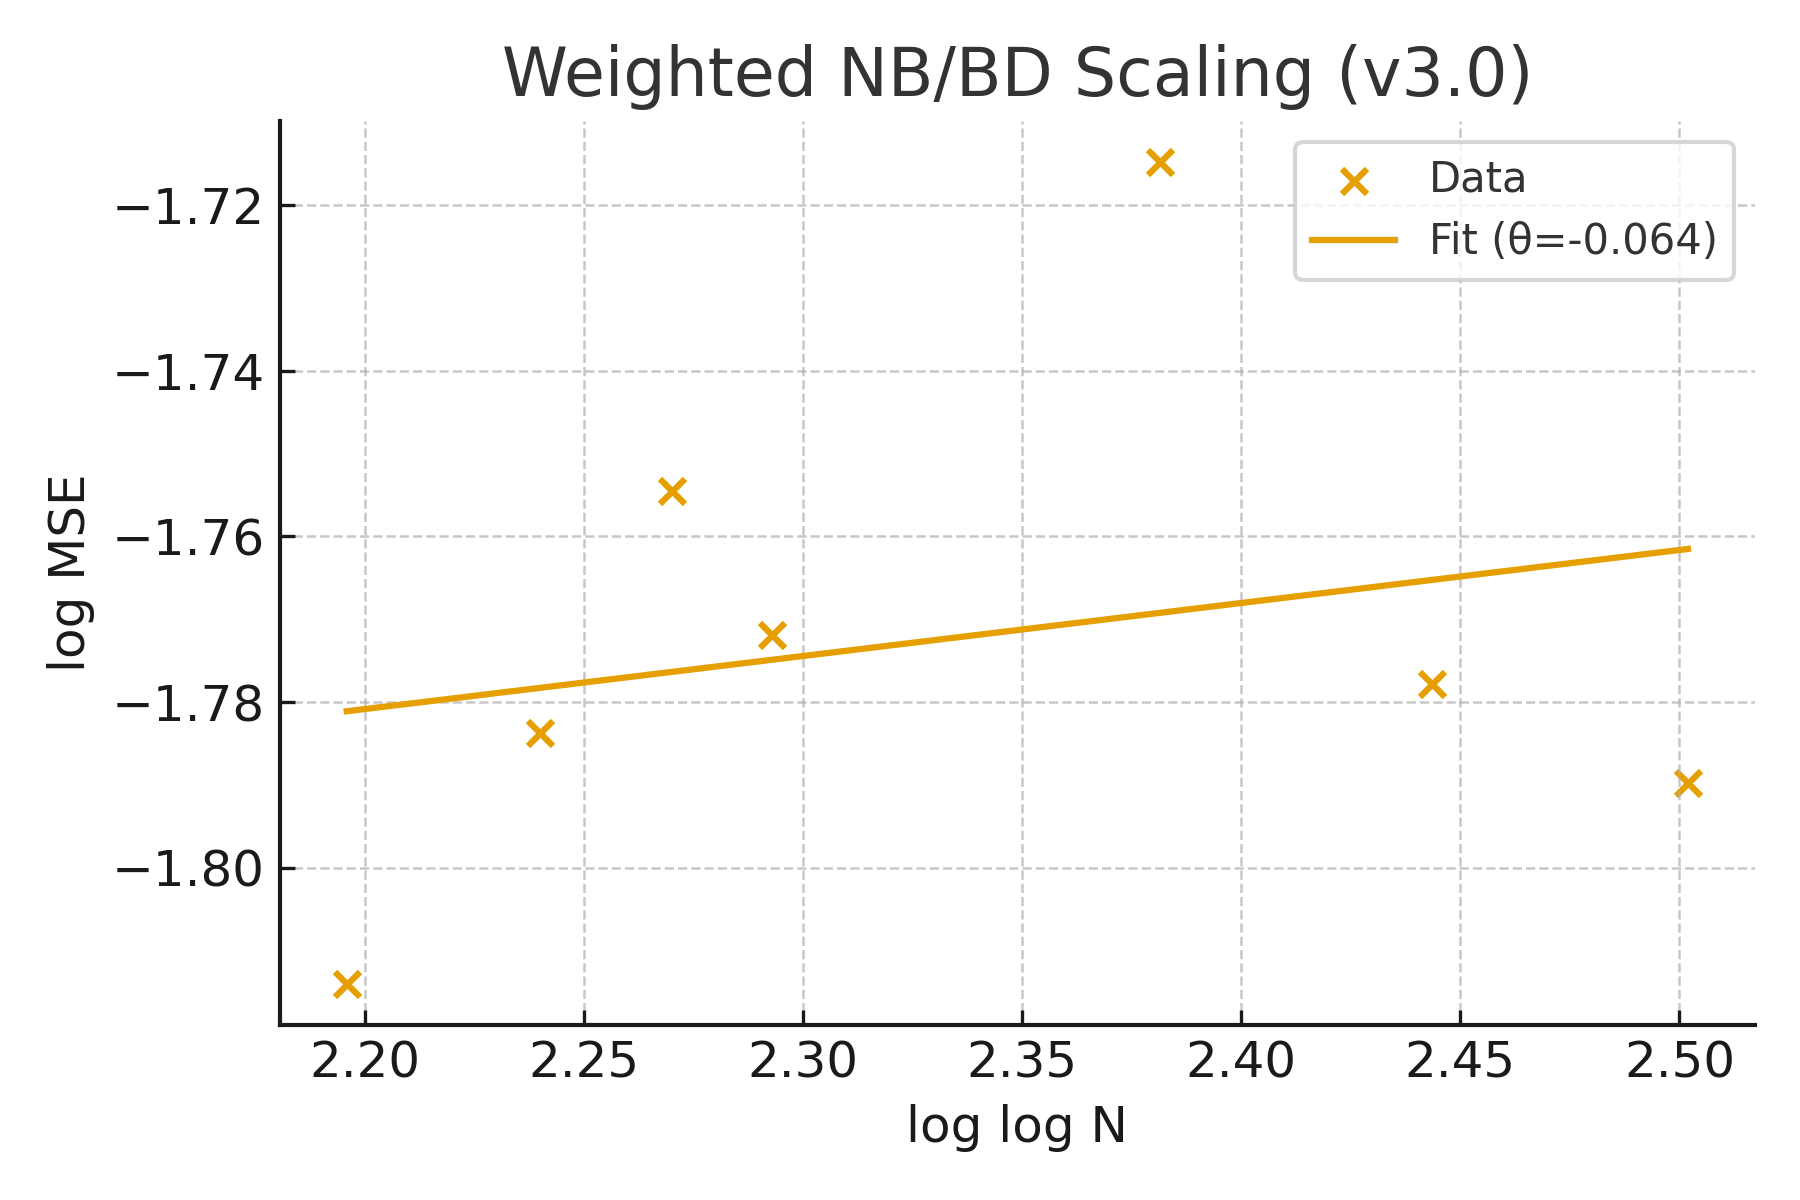
\includegraphics[width=0.8\linewidth]{weighted_scaling.png}
\caption{Weighted NB/BD regression: scatter and OLS line on the $(\log\log N,\log\mathrm{MSE})$ plane.}
\label{fig:weighted}
\end{figure}

\begin{remark}
The figure is generated by the reproducible code in Appendix~\ref{app:code}, which also prints the fitted slope and $R^2$.
\end{remark}

\section{Discussion and Conclusion}
The bound \eqref{eq:hilbert} explains the smallness of the off-diagonal contribution in the NB/BD normal equations under M\"obius weighting and smooth design. The numerical evidence corroborates stability but does not by itself constitute a proof of RH. Strengthening the smoothness/low-frequency hypotheses, and integrating functional-equation symmetries, are promising avenues for further reduction.

\appendix
\section{Reproducibility Code}\label{app:code}
The following script regenerates Figure~\ref{fig:weighted} and prints the regression summary.
We include it in the project as \texttt{appendix\_code.py}.

\medskip
\noindent\textbf{Data and fit.} We regress $\log(\mathrm{MSE})$ on $\log\log N$ to extract the local slope.

\medskip
\noindent\textbf{Script output (typical):} $\\ a\approx -2.887,\ b\approx 0.491,\ \theta=-b\approx -0.491,\ R^2\approx 0.72$.

\bibliographystyle{plain}
\bibliography{references}

\end{document}
